%==============================================================================
%
%      File:  UNHTHESIS.TEX  (Stored in TEX$LATEX: as UNHTHESIS.TEMPLATE)
%  Language:  LaTeX - Document Preparation System
%      Date:  23/Nov/88
%    Author:  Bill Costa
%             USNH Computer Services
%    Updated: Kelly Black
%             Dept. of Math & Stat
%             14 Aug 02
%
%   This document shows how to use the UNHTHESIS latex style sheet to
%   create a thesis.  You will want to make your own copy of this file to
%   get started.  Here are the basic steps:
%
%   Setup LaTeX and the DVI translator.  This makes these programs
%   available for your use, as well as defining library names such as
%   TEX$LATEX:.
%
%        $ SETUP LATEX                  ! Do these commands at the start of
%        $ SETUP DVITOPS/RESET          ! every terminal session (or put them
%        $                              ! in your LOGIN.COM).
%
%   Now copy this template file to your own directory, 
%   Three example chapter files are also included.
%   This step would normally be done only once.
%
%   Follow the instructions below for making the required edits to your
%   own copy of this file.  Once you have created the document you
%   must go through several steps. You must first ``latex'' the file,
%   you view it using xdvi, and when you are done you print it using
%   dvips.
%
%   First to latex your file execute the following command:
%
%        % latex mythesis
%
%   You should fix any errors that are displayed. To view your
%   file you use xdvi:
%
%   % xdvi mythesis
%
%   When you are finally ready to print use dvips:
%
%   % dvips mythesis.
%
%    Revisions:
%    -------------------------------------------------------------------------
%    06-NOV-90 WFC  Uses corrected \documenttype scheme.  See revision notes
%                   in TEX$LATEX:UNHTHESIS.DOC for more details.
%
%------------------------------------------------------------------------------

%    14 Aug 02 Updated document to latex 2e. Also, changed wording 
%              to be consistent with an X windows system.

%    14 Aug 02 Added \includeonly command in comments.

%------------------------------------------------------------------------------
%  Preamble  - You may want to add your own \hyphenation commands.
%------------------------------------------------------------------------------


% During the editing process you will not want to view and print the
% whole document. Uncomment the command below so that only the
% chapters that you want to work on are visible.
%\includeonly{chapter1}

\documentclass[11pt,doublespace]{unhthesis}


% Extra modules can be added to your document to extend the things
% the Latex can Do. One of these is psfig which allows you to print
% postscript files. You tell Latex to read these packages using the
% \usepackage command:

\usepackage{psfig}


\hyphenation{gno-mon-ly}


%------------------------------------------------------------------------------
%  Preliminary Pages - Fill in the `blanks' noted.
%------------------------------------------------------------------------------

\begin{document}
                                                        % TITLE PAGE
                                                        %======================
\title{Creating a Thesis for Fun and Profit}            % Your title
\author{William F. Costa}                               % Your name
\prevdegrees{B.S., Plymouth State College (1976)}       % Your old degree
\major{Computer Science}                                % Your new major
\degree{Master of Science}                              % Your new degree
\degreemonth{May}                                       % When awarded.
\degreeyear{1990}                                       %
\thesisdate{January 10, 1989}                           % Date of document.
\DOCUMENTtype{THESIS}                                   % or DISSERTATION
\Documenttype{Thesis}                                   % or Dissertation
\documenttype{thesis}                                   % or dissertation
\maketitle
                                                        % COPYRIGHT PAGE
                                                        %======================
\copyrightyear{1989}                                    % Delete these
\makecopyright                                          % if no copyright
                                                        % page.

                                                        % APPROVAL PAGE
                                                        %======================
\supervisor{A. B. Smith}{Associate Professor of xxx}    % <- One of these
\committee{A. B. Jones}{Associate Professor of xxx}     % <- As many as
\committee{A. B. Black}{Faculty in Residence in xxx}    %    you need...
\makeapproval                                           %

                                                        % DEDICATION PAGE
                                                        %======================
\begin{dedication}                                      % Delete these
    To Mom and Dad.                                     % if no dedication
\end{dedication}                                        % page.


                                                        % ACK. PAGE
                                                        %======================
\begin{acknowledgments}                                 % Delete these if
     A number of people have made this paper possible.  % no acknowledg.
     In particular                                      % page.
     I wish to thank...                                 %
\end{acknowledgments}                                   %

                                                        % FOREWORD PAGE
\begin{foreword}                                        %======================
     This is the foreword.                              % Delete these if
\end{foreword}                                          % no foreword page.

                                                        % OTHER PAGES
                                                        %======================
\tableofcontents                                        % Always needed...
\listoftables                                           % Delete if no tables.
\listoffigures                                          % Delete if no figures.


%------------------------------------------------------------------------------
%  Document body - Place text into individual include files, such as
%                  as "chap1.tex", or replace each "\include{}" statement
%                  with your actual document text.
%------------------------------------------------------------------------------

                                                % ABSTRACT PAGE
                                                %==============================
\begin{abstractpage}                            % Creates the abstract page.
   Thesis and dissertation creation is hard     %   Your text goes here. Just
   work and a poor graduate student needs all   %   follow the rules given in
   the help he or she can get.  This thesis     %   the LaTeX manual on how to
   attempts to show how \LaTeX can be used to   %   enter/format text using
   make the process just a little bit easier.   %   LaTeX commands.
\end{abstractpage}                              % This ends the page.

                                                % CHAPTERS
                                                %==============================
\include{chapter1}                              % The best way to organize your
% See UNHTHESIS.TEMPLATE for additional comments about this file.
%
\chapter{My Second Chapter Title}

    Remember that, when entering text for your document, you tell LaTeX to
    start a new paragraph by simply inserting a blank line.  Also remember
    that it makes no difference     how      many        spaces      you
    put                   between            words.  One is as good as a
    hundred.

    Do you have a copy of the LaTeX manual~\cite{The-Manual} yet?    You
    {\em will\/} need it.  LaTeX is easy to use and for simple  documents,
    you could probably go a long ways without having to look at the manual. 
    But a thesis or dissertation is not a simple document.  Save yourself
    some grief and get a copy of the manual and start reading it now.
                              % document is probably to keep
                                                % in its own file.  



%------------------------------------------------------------------------------
%  Bibliography and Appendix  - Use the "\cite{}" command in your text
%                               to mark citations, i.e. "\cite{Hans80}".
%------------------------------------------------------------------------------

                                                % THE BIBLIOGRAPHY
                                                %==============================
\begin{thebibliography}{XxxxNN}                 %
                                                %
  \bibitem[Hans80]{FirstRef} D. E. Hanson.      % You need one of these for
      {\em The Title of His/Her Book.}          % each citation.  Use an
      Some Publisher Name,                      % \include{mybib} instead 
      Some Big City                             % if you'd rather to keep 
                                                % these in a separate file.
  \bibitem[Lamp86]{The-Manual} L. Lamport.      %
      {\em LaTeX, User's Guide \& Reference     % See the manual to find out
      Manual}                                   % why we had to use a backslash
      Addison-Wesley Publish Company            % character (\) in front of the 
      Reading, Massachusetts                    % ampersand (&).
                                                %

  \bibitem[Abra90]{abrahams} Abrahams, Paul W., 
    Karl Berry, and Kathryn A. Hargreaves.  
    {\em \TeX\ for the Impatient}.  
    Addison-Wesley Publishing Company, 
    Reading MA, USA, 1990.


  \bibitem[Thom92]{thomas} Thomas, George B. Jr., 
    and Ross L. Finney. 
    {\em Calculus and Analytic Geometry}, 
    8$^{th}$\ ed.  
    Addison-Wesley Publishing Company, 
    Reading MA, USA, 1992.

\end{thebibliography}                           %

                                                % THE APPENDIX
                                                %==============================
\appendix                                       % Include appendix files as
  \begin{singlespace}                           % needed or delete this block
  \chapter{Equations}

Some examples of how to insert mathematical expressions is given in
this appendix. The first set of examples focuses on equations. The
second set of examples provides some details on how to work with
arrays. Finally, some examples are given to show how to work with
different symbols.


\section{Equations}
There are two modes in \LaTeX\ that we will use.  The first is text
mode.  This is the default mode and is used to simply typeset this
text.  The second is math mode.  You must explicitly tell \LaTeX\ when
you want to use math mode.  There are two ways to do this.  If you
want to put symbols in with your text you must use math mode, and you
do this by starting math mode using a \$ and ending with another \$.
Symbols such as the $\backslash$\ must be done in math mode.  At the
end of math mode or a slash command I use a slash followed by a space.
This is done to insure that the proper spacing is used by \LaTeX.  I
do not use a slash space when the symbol is followed by punctuation.


% In the next paragraph I will introduce how to start an
% equation environment.  I will also give the proper credit
% to the source.  I will make a citation using the \cite
% command.  The citation that I use is defined at the end
% of this document in the bibliography.  To use a citation
% you must define the label.  Because the definition is at
% the end of the file the first time you use latex you will
% have to run it through twice to make sure the definitions
% are updated.  (This is my one real gripe about latex)

The other way to start math mode is in an equation environment.  There
are different ways to do this but the most common is to use eqnarray
\cite{The-Manual}.  This environment is started and ended in the same way
the document environment is employed.  For example to give the formula
for a straight line I might do it in slope-intercept format
\cite[p. 8]{thomas},
\begin{eqnarray}
y & = & mx + b.
\end{eqnarray}
The \LaTeX\ program will automatically give the equation a number
and center it as well.  Note that I used two ampersands to set off the
$=$\ sign.  This is done to let \LaTeX\ know where to center the
equation \cite{The-Manual}.  This way I can put more equations in the
equation array and keep them properly justified \cite[p. 7]{thomas},
\begin{eqnarray}
y & = & mx + b, \\
y - y_0 & = & m (x - x_0).
\end{eqnarray}
In some situations, I may have a large number of equations but
only want to see one number.  To keep \LaTeX\ from printing out
a number each time use the nonumber command \cite{The-Manual},
\begin{eqnarray}
y       & = & mx + b \\
y - y_0 & = & m (x - x_0). \nonumber
\end{eqnarray}
(The \LaTeX\ program will automatically typeset things for you so 
you can make your life much easier if you line up things in the
text file.  This will make editing much easier.)

I have introduced something here without telling you.  The \LaTeX\ 
program will let you make subscripts and superscripts using the 
carrot and lower bar symbols.  If I want to make a subscript or superscript
with just one letter it can be done as in the equations above.
If I want to make subscripts and superscripts with more letters I
have to let \LaTeX\ know which letters are to be used through the
use of the braces \cite{The-Manual},
\begin{eqnarray}
y_{approximate} & = & m^{guess} x_{known} + b^{guess}.
\end{eqnarray}
When you know these basics you can go on to create great documents.


Another very useful tool is the new command.  Since I am getting
tired of typing out \LaTeX\ whenever I want the Latex symbol
to appear I can define a new command to do it for me.  In this
case I will call this new command $\backslash$lat.
\newcommand{\lat}{\LaTeX} 
Now whenever I want to use the \lat\ symbol life is much easier.


\section{The Array Environment}
Sometimes the mathematical formulas you have are a little more complicated
than the equation for a line.  The equation array environment defines
three columns and will justify the  text in those columns.  For 
example we can have a simple equation,
\begin{eqnarray}
y & = & x^2.
\end{eqnarray}
In this example, the first column contains the $y$, the second column
contains the $=$, and the third column contains the $x^2$.  The \lat\
program will automatically right justify the first column, center the
second column, and left justify the third column \cite{The-Manual}.
There are times when you would like to have more than three columns.
For example, I would like to put a bound on the values for $x$.  Here
an equation is constructed which has four columns: the first is right
justified, the second is centered, the third is left justified, and
the fourth is left justified.  I will use the array environment which
will be nested {\it inside} the equation array environment
\cite{The-Manual},
\begin{eqnarray}
    \begin{array}{rcll}
       y & = & x^2 & x \in [-1,1].
    \end{array}
\end{eqnarray}
After I defined the array, I had to tell \lat\ how many columns
and how they are to be justified.  Once done, I had to tell
\lat\ how the text was to be put in the columns.  The ampersand
symbol is used to distinguish between columns \cite{The-Manual}.

This same method is used to make arrays of numbers.  For example
a matrix is a simple block of numbers (what we do with them is not
quite as simple),
\begin{eqnarray}
    \begin{array}{rrrr}
       1 &  2 &  3 &  4 \\
      11 & 12 & 13 & 14 \\
      21 & 22 & 23 & 24 \\
      31 & 32 & 33 & 34.
    \end{array}
\end{eqnarray}
This looks kind of messy so I would like to spruce things up.  I want
to put braces on each side of the array.  To do this I have to let
\lat\ know where to put the symbol and which symbol to use.  This is
done through the use of the left and right commands \cite{The-Manual},
\begin{eqnarray}
\left[
    \begin{array}{rrrr}
       1 &  2 &  3 &  4 \\
      11 & 12 & 13 & 14 \\
      21 & 22 & 23 & 24 \\
      31 & 32 & 33 & 34
    \end{array}
\right].
\end{eqnarray}
Here I put the left and right commands {\it outside} of the
array.  The character following the command is the character
to be used and they do not have to be the same \cite{The-Manual},
\begin{eqnarray}
\left\{
    \begin{array}{rrrr}
       1 &  2 &  3 &  4 \\
      11 & 12 & 13 & 14 \\
      21 & 22 & 23 & 24 \\
      31 & 32 & 33 & 34
    \end{array}
\right).
\end{eqnarray}
If I do not want a closing character on the right side I must still
let \lat\ know where to close (this will let me do more complicated
things with nested brackets and such).  If there will be no symbol on
one side use a period to let \lat\ know where to end the current
set of delimiters \cite{The-Manual},
\begin{eqnarray}
\left\{
    \begin{array}{rrrr}
       1 &  2 &  3 &  4 \\
      11 & 12 & 13 & 14 \\
      21 & 22 & 23 & 24 \\
      31 & 32 & 33 & 34.
    \end{array}
\right. 
\end{eqnarray}

Using the array environment we can now place an array inside 
one of the columns of another array.  The most common example
of this would be the use of an array in one of the standard
columns of the equation array.  For example, we can now define
$y$\ as a function of $x$\ where the formula to be used depends
on $x$,
\begin{eqnarray}
y & = & \left\{
           \begin{array}{lrcccl}
              x^2           & -1 & < & x & \leq & 0 \\
              \sin(\pi x)   &  0 & < & x & <    & 1.
           \end{array}
        \right.
\end{eqnarray}


\section{Mathematical Symbols}
Other than the low cost of the program, one of the nice things
about the \lat\ program is the ease in which symbols can be 
used in formulas and mixed with text.  In this section I will
try to give a list of some of the symbols you will be using.
First, the commands for the Greek letters are given.  Next,
the commands for mathematical functions are given, and then
various other important symbols are given. This is not a 
complete list but is merely some of the symbols that are most
often used.  For the complete list consult any of the \lat\ 
manuals in the bookstore.

\subsection{Greek Letters}
The \lat\ program will let you display all of the Greek letters
in both lower and upper case.  The lower case letters are displayed
using all lower case letters \cite{The-Manual},
\begin{eqnarray}
    \begin{array}{ccccccc}
       \alpha & \beta     & \gamma    & \delta   & \epsilon & \varepsilon & \zeta \\
       \eta   & \theta    & \vartheta & \iota    & \kappa   & \lambda     & \mu   \\
       \nu    & \xi       & o         & \pi      & \varpi   & \rho        & \varrho \\
       \sigma & \varsigma & \tau      & \upsilon & \phi     & \varphi     & \chi   \\
       \psi   & \omega
    \end{array}
\nonumber
\end{eqnarray}
To use an upper case Greek letter use the same command only the 
first letter should be upper case.  For example, $\Pi$\ is the
upper case version of $\pi$ \cite{The-Manual}.

\subsection{Math Functions}
When printing text in math mode \lat\ uses italic type.  This 
can be a problem when you want to use a function in a formula,
\begin{eqnarray}
y & = & sin(\pi x).
\end{eqnarray}
The letters in the function sine are in italic, and it is hard to tell
the difference between the letters used elsewhere.  To make it easier
to differentiate between the different things in your formulas, \lat\
makes it easy for you to use a different typeset.  The most common
functions that are used have their own \lat\ commands.  Going back to
our example, we can let the reader know the difference between the
variables and the functions,
\begin{eqnarray}
y & = & \sin( \pi x).
\end{eqnarray}
(I used a space between the command to make $\pi$\ and the $x$.
When in math mode \lat\ will print things out without the spaces.)

Other functions that have \lat\ commands are listed below \cite{The-Manual},
\begin{eqnarray}
   \begin{array}{lllllll}
      \arccos & \arcsin & \arctan & \cos    & \cosh   & \cot & \coth \\
      \csc    & \exp    & \lim    & \liminf & \limsup & \ln  & \log  \\
      \max    & \min    & \sec    & \sin    & \sinh   & \sup & \tan \\
      \tanh
   \end{array}
\end{eqnarray}

\subsection{Math Symbols}
Besides the Greek letters and the various math functions, the \lat\ 
program has many symbols.  Here a very brief list of these symbols
is given \cite{The-Manual}.  For a more complete list please see one of the \lat\ 
books in the bookstore.

\begin{eqnarray}
   \begin{array}{lllllll}
      \pm     & \times  & \div      & \cap    & \cup   & \triangle & \leq \\
      \subset & \in     & \geq      & \supset & \equiv & \approx   & \neq \\
      \propto & \perp   & \parallel & \smile  & \frown & \imath    & \jmath \\
      \Re     & \Im     & \prime    & \nabla  & \angle & \forall   & \infty \\
      \sum    & \int    & \partial
   \end{array}
\end{eqnarray}




\subsection{Putting it Together}
Once you know how to put different symbols in your document the \lat\ 
program has a few tools that will let you combine things and display
different operations.  For example, \lat\ will let you write things
as a fraction.  This is done with the frac command which takes two
arguments \cite{The-Manual}.  The first argument is the numerator and the second operator
is the denominator.  The different arguments are set apart using braces,
\begin{eqnarray}
   y & = & \frac{\sin(x)}{x}.
\end{eqnarray}

Other symbols may require more information than just the symbol.  For
example, when using the sum symbol, ($\sum$), you have to let your
reader know where to start adding and when to stop.  Since these
arguments are found above and below the symbols they are added through
the use of superscripts and subscripts,
\begin{eqnarray}
   \sum^{N}_{i=0}  \left( \frac{1}{s} \right)^i
             & = & \frac{1 - \left( \frac{1}{s}\right)^{N+1}}
                        {1-\frac{1}{s}}
\end{eqnarray}
As you can see, some of the formulas you use require you to use
operations that are nested within operations.  The formulas you use
can become quite complicated in short order.  When you type these
formulas in it will be to your advantage to do so carefully and to
make them readable.  Otherwise, you may be in for some long nights
in the computer center!

Another symbol that you will use is the integral symbol,
\begin{eqnarray}
\int        x dx & = & \frac{1}{2} x^2 + c \\
\int^1_{-1} x dx & = & 0. \nonumber
\end{eqnarray}
The limits are added using superscripts and subscripts.
One problem with the formulas above is that \lat\ likes
to run everything together in math mode.  When you want a
space in a formula you must explicitly tell \lat\ where
to put the space.  This is done with the same command
used while in text mode \cite{The-Manual},
\begin{eqnarray}
\int^1_{-1} x \ dx & = & 0.
\end{eqnarray}


Another function that may prove useful is the square
root function \cite{The-Manual},
\begin{eqnarray}
\sqrt{x^3} & = & x^{\frac{3}{2}}. 
\end{eqnarray}

Finally, another useful thing is to put one symbol
over another without the bar you see in fractions.
This is done using stackrel \cite{The-Manual}. 
$\stackrel{\circ \circ}{\smile}$

\subsection{Remembering Equation Numbers}
When you have equations in your document you will most likely want to
refer to the equations in the text.  Rather than trying to figure out
what each equation number is \lat\ will let you put a label on an
equation and refer to the label \cite{The-Manual}.  This way, when you
add and delete equations as your document ferments you will not have
to go back and change equation numbers.  I will give some examples of
how this is done and then will let you know the dangers.

First, to refer to an equation you must first put a label on the
equation,
\begin{eqnarray}
\label{derivative}
f'(x) & = & \frac{d}{dx} \left( x \sin(x) \right).
\end{eqnarray}
Once labeled, I can easily refer to equation (\ref{derivative}).
To make the reference look like the original equation I had
to put the parenthesis around the reference myself.  It is
considered bad form if your reference does not look like the
original.  

There are some warnings that should be heeded.  The way that \lat\
numbers things can be a little quirky.  The \lat\ program keeps a
running tab of the current equation number.  When it meets an
equation that does not have a nonumber command it assigns the current
number to the equations and {\em then} increments the equation number
\cite{The-Manual}.  So if I have an equation with two lines I have to put
the label in the right place,
\begin{eqnarray}
\label{thereallabel}
\frac{d}{dx} f(x) & = &  x \sin(x), \\
f(x)  & = & -x \cos(x) + \sin(x).
\label{antiderivative}
\nonumber
\end{eqnarray}
Now when I want to say something about (\ref{antiderivative})
I might not get the right number! However, if I refer to
equation (\ref{thereallabel}) I will get the correct number.

There is one other thing that you should keep in mind.  The \lat\
program is a bit primitive in the way that it remembers things.  The
program must keep tabs of the equation numbers so that when you refer
to them it can use the equation number.  Because you might want to
refer to an equation before it is given, the \lat\ program must play
some book-keeping tricks.  To do this the program creates a file {\em
after} you run your document through the program.  Then the {\em next}
time you use \lat\ it can figure out what equation numbers to use.
When you make changes that involve the numbering of the equations you
may have to run your document through \lat\ twice to get it right.  No
one ever said that life would be easy $\ldots$
                          % of lines if no appendix.
  \chapter{Figures}

Tables are nice, but printing a postscript file in with your text is
more important (in my own humble opinion).  Fortunately, \LaTeX will
let you do this.  Here I am using the psfig command to print the
picture.  It will automatically read the plot, figure out how big it
is and print it out.  You should be careful since this is not a
``standard'' feature.  The psfig command is something that somebody
else added since it is very useful.  The bad news is that not
everybody has this little gem.  Because it is so useful most
installations do have it.  If you find yourself using a version that
does not you should complain until somebody installs it.  It is far
too useful!


If you don't believe me just look at Figure \ref{twodtest}.  It
certainly is a fine picture.  I could look at it all day $\ldots$ One
quick note for UNH is in order here.  If you include a postscript
picture you {\em cannot} print it on the text printer using the dvi
options.  You must print it on the postscript printer and use dvips to
do so.

One other quick note about some maple postscript files.  If you use a
postscript file generated by some versions of maple, psfig may not
give you the correct size.  This is because some versions of maple do
not create a proper encapsulated postscript file (say that three times
fast).  If you have a maple plot and it does not print out correctly
using psfig you will have to edit the file.  To make things right edit
the file and replace the line with the bounding box so that it looks
like this,
\begin{verbatim}
%%BoundingBox:  0 0 612 792
\end{verbatim}
This line is about 6 or 7 lines from the top.


\begin{figure}[htbp]
\centerline{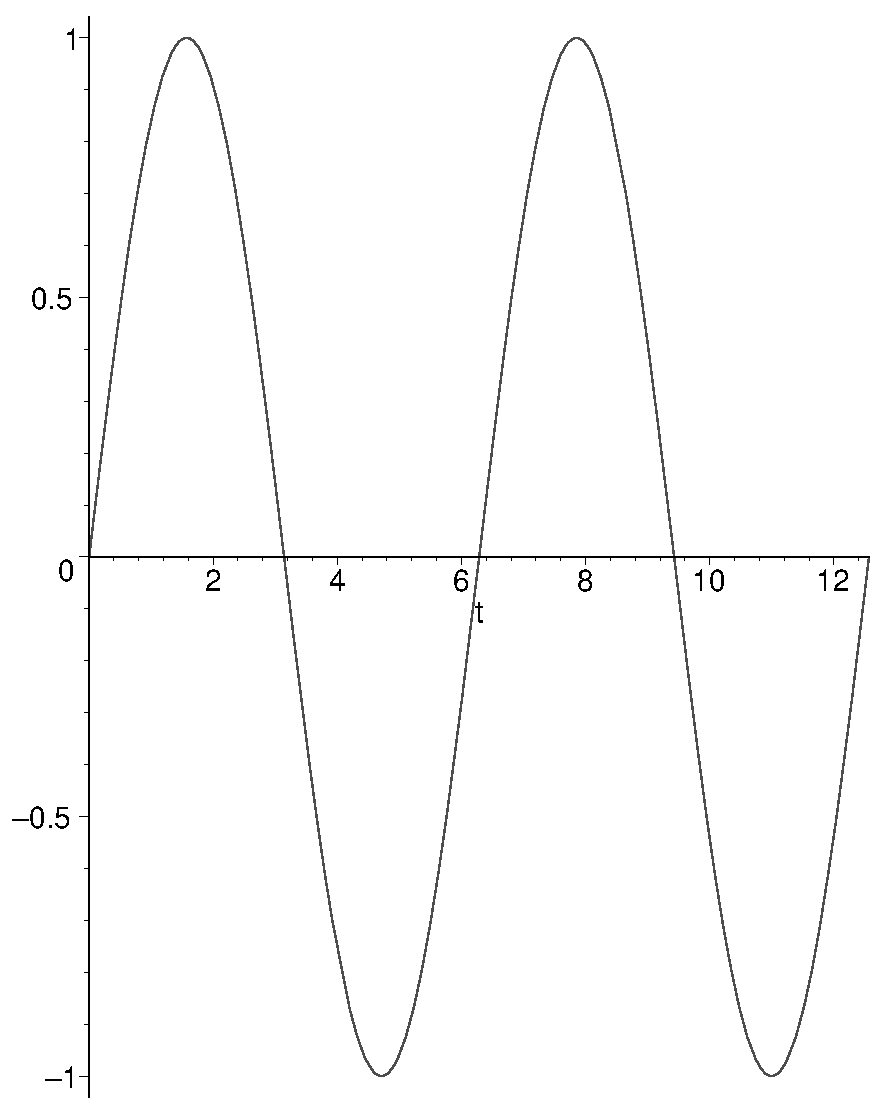
\psfig{file=sine.eps,height=3.0in}}
\caption{This here is a figure of a curve.}
\label{twodtest}
\end{figure}

                          %
  \chapter{Misc. Ramblings}

Like any piece of software \LaTeX has its shares of quirks and little
odds and ends. Here I will share a few notes on lists and finally add
some comments on some of the commands that I have found to be useful.

\section{Lists}

I have already given an example of one kind of list using the
itemize environment.  A complete list is given below \cite{The-Manual}:
\begin{enumerate}
\item The itemize list.
\item An enumerate list.
\item A description list.
\end{enumerate}
The different types of lists are described below 
\cite[p. 65]{The-Manual}:
\begin{description}
\item[itemize]     Lists each item with a $\bullet$.
\item[enumerate]   Gives a numbered list.
\item[description] Used to describe the members of a list.
\end{description}


You can also put a list inside a list.  If you use
enumerate it will even keep track of the numbers for you:
\begin{enumerate}
\item Top Five Reasons to take Calculus:
    \begin{enumerate}
     \item Annoy roommate when pulling all-nighters.
     \item At 8:00AM it's too dark for volleyball.
     \item Three words: The chain rule.
     \item Can learn how to use $\Sigma$\  without 
           referring to alcohol.
     \item Can impress date with knowledge of the limit.
     \end{enumerate}
\item Top Five Worst Reasons to take Calculus:
     \begin{enumerate}
     \item Would like to learn how to use that spiffy calculator.
     \item If you have to spend a lot of money on a book it should
             at least be a really thick book, damnit.
     \item Would like to learn new French and German names to
             impress people at parties.
     \item Satisfies the liberal arts school's requirement
           for ``class that requires that you know how to  count''.
     \item Morning class is motivation to go get breakfast 
           before they run out of those pancakes.
     \end{enumerate}
\end{enumerate}


\section{Window Dressings}
Since some of you may actually like having a typesetting
program around, I thought I might like to share some
of the little things that help round out the \lat\ program.
For example, I often use \lat\ for letters.  When I want
to write one of my colleagues, Einar Ronqui\o st, I need
to know how to use some extra characters.  Other non-English
characters include the following: \oe, \OE, \ae,
\AE, \aa, \AA, \o, \O, \l, \L, \ss,
?`, !`.

People from foreign lands also like to use accents which
are not included on the standard keyboard.  To get around
this \lat\ has some commands for \`{a}ccents.  See Table
\ref{accents} for a list \cite[p. 40 (blatant rip-off)]{The-Manual}
and Table \ref{mathaccents} for a list of accents for use
in math mode \cite[p. 51]{The-Manual}.

\newcommand{\bs}{$\backslash$}
\begin{table}[hbpt]
\begin{tabular}{r @{-} l @{\hspace{0.5in}} r @{-} l  @{\hspace{0.5in}}
                r @{-} l @{\hspace{0.5in}} r @{-} l }
\`{a} & \bs `\{a\} & 
\~{a} & \bs \~\{a\} & 
\v{a} & \bs v\{a\} & 
\c{o} & \bs c\{o\}  \\
\'{a} & \bs '\{a\} & 
\={a} & \bs =\{a\} & 
\H{a} & \bs H\{a\} & 
\d{o} & \bs d\{o\}  \\
\^{a} & \bs \^\{a\} & 
\.{a} & \bs .\{a\} & 
\t{aa} & \bs t\{aa\} & 
\b{o} & \bs b\{o\}  \\
\"{a} & \bs "\{a\} & 
\u{a} & \bs u\{a\} 
\end{tabular}
\caption{Some accents for you to use.}
\label{accents}
\end{table}

\begin{table}[hbpt]
\begin{tabular}{r @{-} l @{\hspace{0.5in}} r @{-} l  @{\hspace{0.5in}}
                r @{-} l @{\hspace{0.5in}} r @{-} l }
$\hat{u}$   & \bs hat\{u\} & 
$\acute{u}$ & \bs acute\{u\} & 
$\bar{u}$   & \bs bar\{u\} & 
$\dot{u}$   & \bs dot\{u\}  \\
$\check{u}$ & \bs check\{u\} & 
$\grave{u}$ & \bs grave\{u\} & 
$\vec{u}$   & \bs vec\{u\} & 
$\ddot{u}$  & \bs ddot\{u\}  \\
$\breve{u}$ & \bs breve\{u\} & 
$\tilde{u}$ & \bs tilde\{u\}
\end{tabular}
\caption{Some accents for you to use in math mode.}
\label{mathaccents}
\end{table}

                          %
\end{singlespace}                               %


\end{document}                                  % Ends the entire document...
